% ------------------------------------------------------------------------------
% TYPO3 CMS 8 LTS - What's New - Chapter "Backend User Interface" (Dutch Version)
%
% @author	Michael Schams <schams.net>
% @license	Creative Commons BY-NC-SA 3.0
% @link		http://typo3.org/download/release-notes/whats-new/
% @language	English
% ------------------------------------------------------------------------------
% LTXE-CHAPTER-UID:		a4c76099-c7aef102-9c114217-0e87f17d
% LTXE-CHAPTER-NAME:	CKEditor
% ------------------------------------------------------------------------------

\section{Rich Text Editor}
\begin{frame}[fragile]
	\frametitle{Rich Text Editor}

	\begin{center}\huge{\color{typo3darkgrey}\textbf{Rich Text Editor}}\end{center}
	\begin{center}\large{\textit{Tekstverwerking neemt een grote stap voorwaarts}}\end{center}

\end{frame}

% ------------------------------------------------------------------------------
% LTXE-SLIDE-START
% LTXE-SLIDE-UID:		537cc1d8-0bd1863d-afd05b05-ab50cc45
% LTXE-SLIDE-ORIGIN:	9d35effa-86de2791-6e57298b-bf673c19 English
% LTXE-SLIDE-TITLE:		CKEditor: Quick Facts
% ------------------------------------------------------------------------------
\begin{frame}[fragile]
	\frametitle{Rich Text Editor}
	\framesubtitle{CKEditor integratie}

	\begin{itemize}

		\item Nieuwe tekstverwerker (RTE) ingebouwd: \textbf{CKEditor}
		\item Bekend en veel gebruikt in PHP projecten, eenvoudig te configureren
		\item Vervangt "HtmlArea" en vormt de basis voor toekomstig bewerken in frontend
		\item HtmlArea is nog beschikbaar als optionele extensie in de TYPO3 Extension Repository (TER)

		\item Crowdfunding actie gestart door de Zweedse agency
			\href{http://pixelant.net}{Pixelant AB} bracht meer dan
			63.000,- Euro (110+ supporters wereldwijd) op

	\end{itemize}

\end{frame}

% ------------------------------------------------------------------------------
% LTXE-SLIDE-START
% LTXE-SLIDE-UID:		b3d1df30-cba7ac93-791b929e-3995191f
% LTXE-SLIDE-ORIGIN:	e99e7216-970412d5-5614a450-364ddba8 English
% LTXE-SLIDE-TITLE:		CKEditor Integration
% ------------------------------------------------------------------------------
\begin{frame}[fragile]
	\frametitle{Rich Text Editor}
	\framesubtitle{Screenshots}

	\begin{columns}[T]
		\begin{column}{.5\textwidth}
			\begin{figure}\vspace*{-0.4cm}
				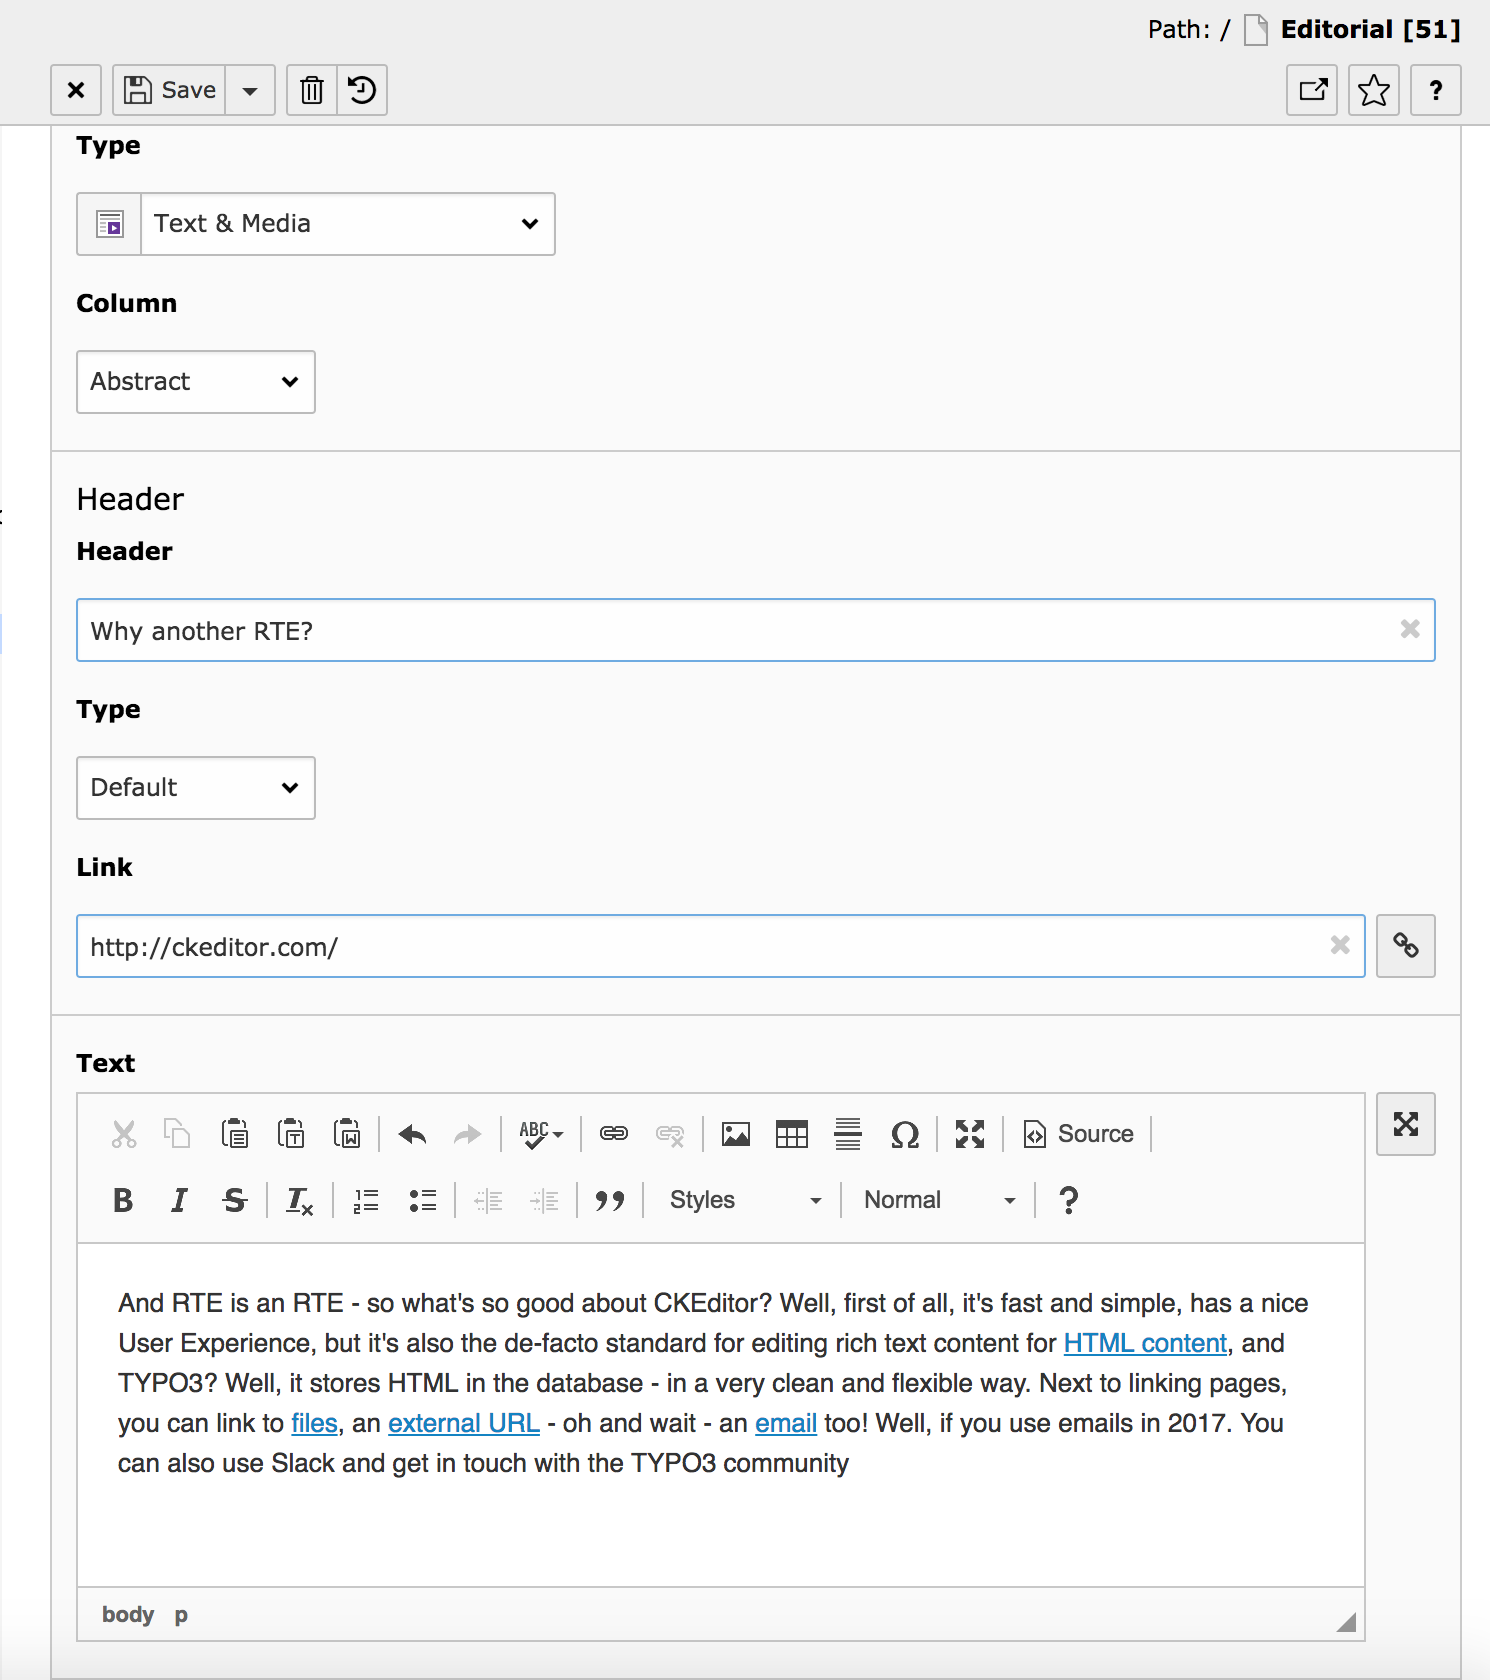
\includegraphics[width=0.8\linewidth]{CKEditor/ckeditor-1.png}
			\end{figure}
		\end{column}
		\begin{column}{.5\textwidth}
%			\begin{figure}\vspace*{-0.4cm}
%				
\includegraphics[width=0.8\linewidth]{CKEditor/ckeditor-2.png}
%			\end{figure}
		\end{column}
	\end{columns}

\end{frame}

% ------------------------------------------------------------------------------
